\chapter{Projective Geometry} \label{chapter:projective_geometry}
This chapter presents the theoretical concepts in projective geometry which are necessary to perform measurements from an image.
First, an introduction to projective geometry is given.
Then follows the projective camera model and planar homographies, which provide the equations which will be used to make measurements.
Then follows a description of camera calibration, which is the process of gathering the necessary information about unknown cameras, so that these equations can be used. 
First offline calibration is described, which is used to created the baseline implementation.
Then, vanishing point calibration is described, which is used to calibrate a camera online, from a single view.

\section{Introduction}
Everyone has a basic understanding of how projective geometry works.
We experience it at every wake moment, without thinking about it. 
The perceived shape of an object can be very different, depending on from where it is viewed.
The square and circle in figure \ref{fig:circle} turn into an ellipse and a trapezium when viewed from a different perspective in figure \ref{fig:circle_perspective}.
The two images are related by a \textit{projective transformation}.
Projective geometry describes these kinds of phenomena.

\begin{figure}
	\centering
	\begin{subfigure}[b]{0.4\textwidth}
		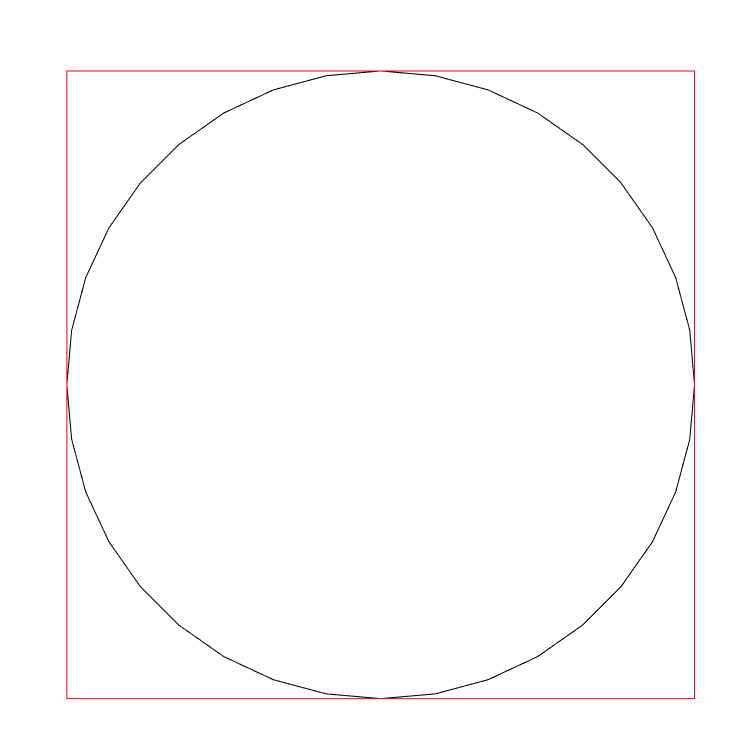
\includegraphics[width=\textwidth]{figures/circle.png}
		\caption{}
		\label{fig:circle}
	\end{subfigure}
	~~~
	\begin{subfigure}[b]{0.4\textwidth}
		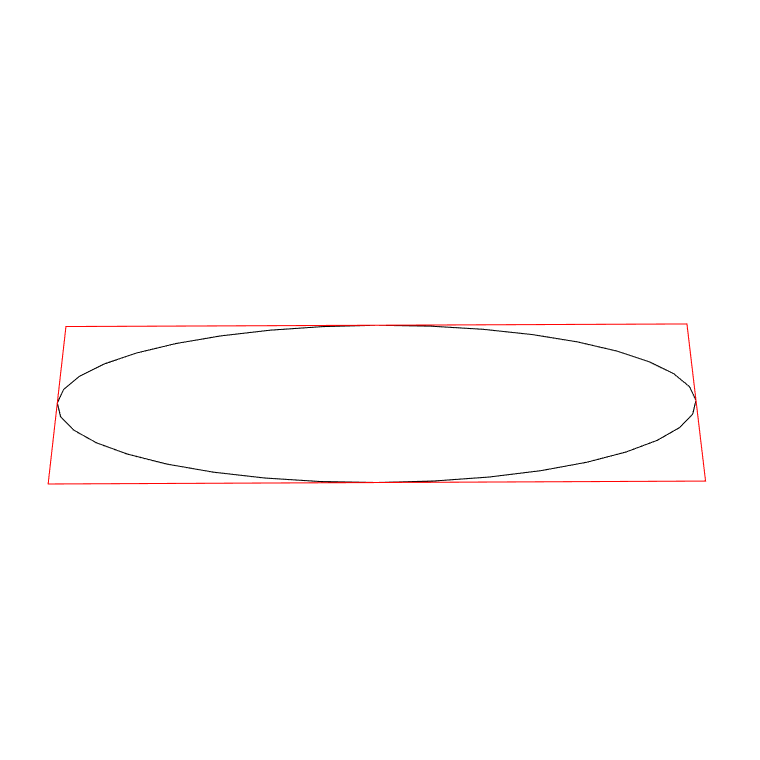
\includegraphics[width=\textwidth]{figures/circle_perspective.png}
		\caption{}
		\label{fig:circle_perspective}
	\end{subfigure}
		\caption{(a) A circle enclosed by a square. (b) The same circle and square, distorted by a projective transformation.}\label{fig:perspective}
\end{figure}

As can be seen in figure \ref{fig:perspective}, very little is preserved by a projective transformation.
Neither shape, lengths, angles, distances, or ratios of distances are preserved.
It turns out that the most general property in a scene that is preserved by a projective transformation is straightness \cite[p. 1]{hartley-zisserman}.

\section{Homogeneous coordinates}

In Euclidean geometry, a point in two-dimensional space is typically represented by cartesian coordinates.
In projective geometry, the homogeneous coordinate system is used instead.
To convert the Cartesian coordinate pair $(x,y)$ to homogeneous coordinates, a one is appended to the cartesian coordinates, resulting in the point $(x,y,1)$. 
Conversely, the cartesian representation of the homogeneous point $(\tilde{x},\tilde{y},\tilde{z})$ is $(\tilde{x}/\tilde{z},\tilde{y}/\tilde{z})$. 
In other words, homogeneous coordinates ignore scale; $(x,y,1)$ and $(kx,ky,k)$ represents the same point for any nonzero value $k$.
These principles extend to other dimensions as well \cite[p. 2]{hartley-zisserman}.

Figure \ref{fig:central_projection_camera} can help to give an intuitive understanding of homogeneous coordinates.
The homogeneous point $\textbf{X}$ and the corresponding cartesian point $\textbf{x}$ in the image plane, lie on the same ray which originates from the camera centre.
Regardless of how $\textbf{X}$ is scaled, it will still correspond to the same point in the image plane.

\section{The projective camera model}\label{camera-model}
Cameras create a 3D projection of the world, i.e. a mapping of 3D coordinates to a 2D plane.
Homogeneous coordinates provide an elegant way to perform this mapping, with a model called the projective camera model.
It is based on a pinhole camera model, where all rays of light pass through a single point called the camera centre, $C$. Before reaching $C$, each ray will pierce the image plane, where the image is projected.
Its location is determined by $f$, the focal length of the camera.

\begin{figure}
\begin{center}
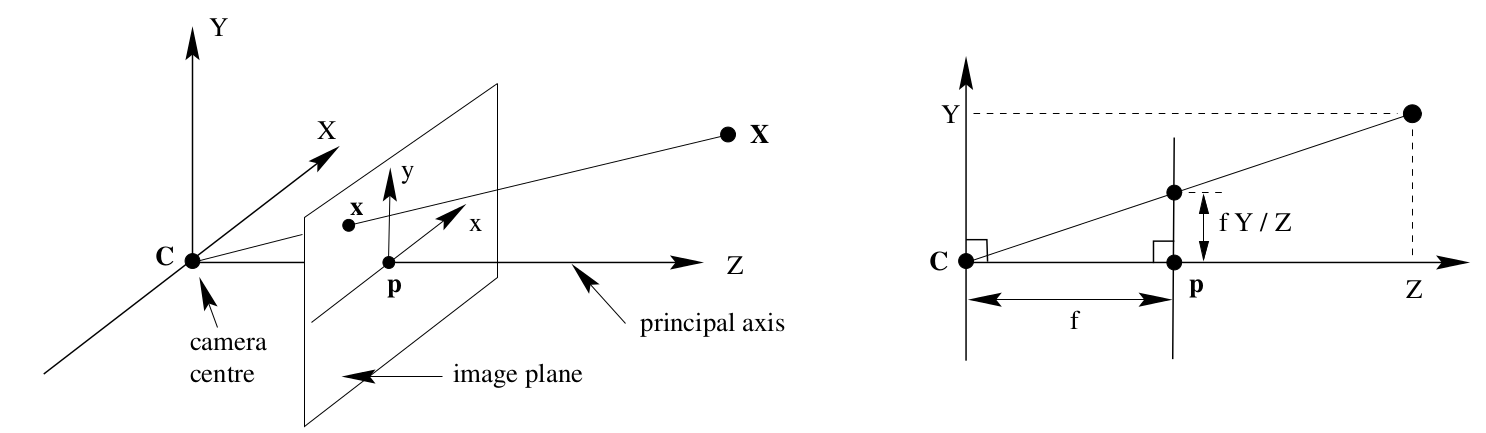
\includegraphics[width=1.0\textwidth]{figures/central_projection_camera.png}
\end{center}
\credit{\cite[p. 154]{hartley-zisserman}}
\caption[The projective camera model]{The central projection camera model. This is a simplification of the general projective camera model, where the image plane is placed with offset $f$ on the $Z$ axis but is otherwise aligned with the world coordinate system.}
\label{fig:central_projection_camera}
\end{figure}

Using the central projection model, as shown in figure \ref{fig:central_projection_camera}, a 3D point can be mapped to a 2D image point, using this simple mapping: $$(X,Y,Z)^T\mapsto(fX/Z,fY/Z)^T.$$
The central projection model makes some rather limiting assumptions, which we will now generalise.
First, the origin of the image coordinate system is not necessarily in the centre.
To remedy this, an offset to the principal point, $(p_{x}, p_{y})$, is added, which represents the coordinates of the centre of the image.
Furthermore, the mapping above assumes that the camera is not rotated, and located in the origin of the world coordinate system. Taking this into account, the following equation can be formed:
\begin{equation}\label{eq:projection1}
\begin{pmatrix}	\tilde{u}\\\tilde{v}\\\tilde{w}\end{pmatrix} = 
\begin{pmatrix}
	f & 0 & p_{x}\\
	0 & f & p_{y}\\
	0 & 0 & 1
\end{pmatrix}
\begin{pmatrix}
	r_{11} & r_{12} & r_{13} & t_{1}\\
	r_{21} & r_{22} & r_{23} & t_{2}\\
	r_{31} & r_{32} & r_{33} & t_{3}
\end{pmatrix}
\begin{pmatrix}	X\\Y\\Z\\1\end{pmatrix},
\end{equation}

where $(\tilde{u},\tilde{v},\tilde{w})^T$ are the homogeneous coordinates of the pixel in the image of the world coordinates $(X,Y,Z)$.
As explained earlier, the cartesian coordinates are obtained by dividing by $\tilde{w}$:
$$
u = \frac{\tilde{u}}{\tilde{w}},~~v = \frac{\tilde{v}}{\tilde{w}}.
$$
The above is the projective camera model that will be used in this thesis. 
It can be generalised further to take things like non-square, or skewed pixels, but that is left out, since the shape of pixels is typically very close to square.

The left matrices in equation \ref{eq:projection1} is called the intrinsic matrix, $K$.
Its entries, the intrinsic parameters, depend only on the camera, and are always the same for a given camera, if there is no change in zoom.
The right matrix is called the extrinsic matrix, which contains the extrinsic parameters of the camera.
The extrinsic parameters are not tied to the camera's properties, but depend on where in the world coordinate system the camera is located, and where it points.
Equation \ref{eq:projection1} can also be written in the more concise form $x = K[R|t]X$.

When multiplied together, the intrinsic and extrinsic matrices form a $3\times4$-matrix, called the camera matrix, $P$:
\begin{equation} \label{eq:projection2}
\begin{pmatrix} \tilde{u} \\ \tilde{v} \\ \tilde{w} \end{pmatrix} =
\begin{pmatrix} p_{11} & p_{12} & p_{13} & p_{14} \\
 				p_{21} & p_{22} & p_{23} & p_{24} \\
				p_{31} & p_{32} & p_{33} & p_{34} \end{pmatrix}
\begin{pmatrix}X \\Y \\Z \\1\end{pmatrix}.
\end{equation}
$P$ is a homogeneous matrix, and thus only has 11 degree of freedom.
Assuming that $P_{34}$ is nonzero, the above can be written as:
\begin{equation}\label{eq:projection3}
\begin{pmatrix} \tilde{u} \\ \tilde{v} \\ \tilde{w} \end{pmatrix} =
\begin{pmatrix} p_{11} & p_{12} & p_{13} & p_{14} \\
 				p_{21} & p_{22} & p_{23} & p_{24} \\
				p_{31} & p_{32} & p_{33} & 1 \end{pmatrix}
\begin{pmatrix}X \\Y \\Z \\1\end{pmatrix},
\end{equation}
where the scaling of the elements of $P$ is implicit \cite[p. 153-165]{hartley-zisserman}.

\section{Planar homographies}\label{planar-homographies}
Assume that a projective camera is observing a planar scene, and that we would like to map points on the plane to points on the image plane. 
If the world coordinate system is defined so the plane is the plane $Z=0$, the projective camera model can be simplified by removing the $Z$ coordinate and the the third column of $P$ from equation \ref{eq:projection3}. 
This scenario, which is depicted in figure \ref{fig:planar_homography}, yields the following system:
\begin{equation}\label{eq:homography}
\begin{pmatrix} \tilde{u} \\ \tilde{v} \\ \tilde{w} \end{pmatrix} =
\begin{pmatrix} h_{11} & h_{12} & h_{13}  \\
 				h_{21} & h_{22} & h_{23}  \\
				h_{31} & h_{32} & 1\end{pmatrix}
\begin{pmatrix}X \\Y \\ 1\end{pmatrix}.
\end{equation}

\begin{figure}
\begin{center}
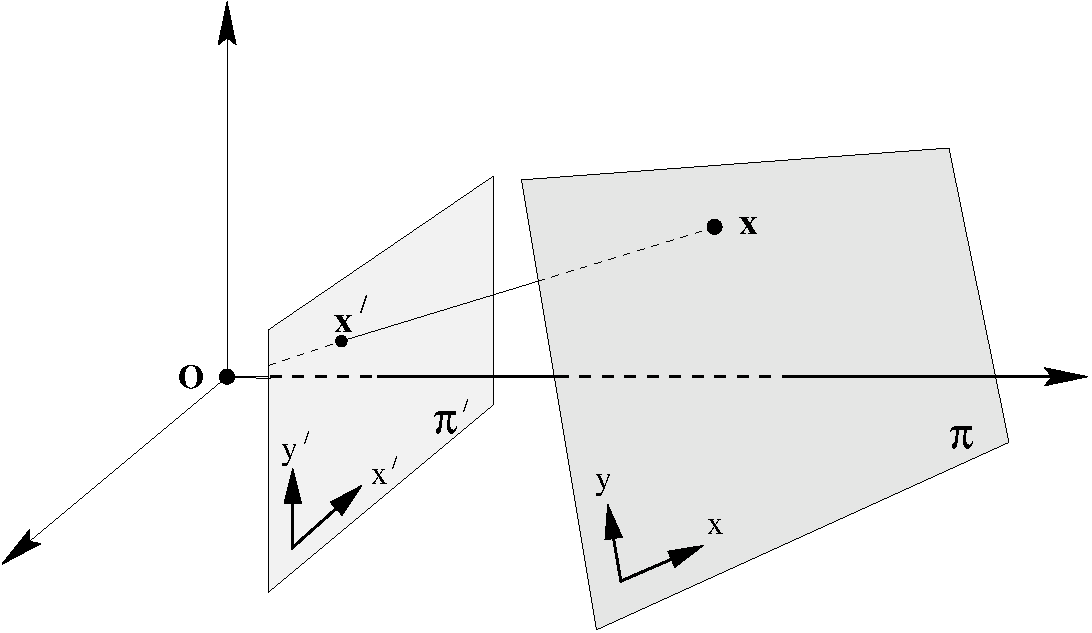
\includegraphics[width=1.0\textwidth]{figures/planar_homography.pdf}
\end{center}
\credit{\cite[p. 34]{hartley-zisserman}}
\caption[Illustration of planar homographies]{A point on a plane in the world is projected to the image plane. A planar homography can be used to map points between the two planes.}
\label{fig:planar_homography}
\end{figure}

This transformation is called a planar homography. The homography matrix, $H$ has 8 degrees of freedom. 
This is a linear equation system, meaning that $H$ can be determined with 8 linear equations.
A pair of known corresponding points on the two planes, $x=HX$ will each contribute with two linear equations to constrain $H$.
Thus, four known corresponding points are required to fully determine $H$.
This assumes that each point contributes with a unique equation.
If three or more of the points in a minimal solution are collinear, a unique solution cannot be determined.
Such a configuration is \textit{degenerate} \cite[p. 91-92]{hartley-zisserman}. 

Since the positions of the corresponding points are typically noisy, an exact solution can often not be found.
One method to find a solution with minimal error is the Direct Linear Transformation algorithm (DLT) \cite{homography-estimation}. 

\section{The plane at infinity and the absolute conic} \label{ac}
Two critical concepts in projective geometry are the plane at infinity, $\pi_{\infty}$ and the absolute conic, $\omega_{\infty}$.
These are very theoretical concepts and will only be touched upon briefly due to their importance for camera calibration.

As mentioned earlier, parallelism is not preserved by projective transformations. 
As a consequence, lines that are parallel in euclidean space are not necessarily parallel in projective space, but intersect at a vanishing point.
An example of this is how parallel train tracks meet at the horizon.

$\pi_{\infty}$ is a plane in which parallel lines meet. 
On $\pi_{\infty}$ lies an imaginary conic, the absolute conic, $\omega_{\infty}$.
Its projection onto the image plane is called the Image of the Absolute Conic.
The full theory regarding these concepts is out of scope for this thesis, but the important thing to know is that $\omega_{\infty}$ is invariant to projective transformations.
This has important implications for camera calibration, because it means that $\omega_{\infty}$ acts as a natural calibration object present in every image.
It can be shown that the following relationship exists between $K$ and the image of the image of the absolute conic:
\begin{equation}\label{eq:conic_k}
	\omega = (KK^T)^{-1}
\end{equation}
\cite[p. 210]{hartley-zisserman}. 

\section{Camera calibration} \label{camera-calibration}
This section describes how to determine the camera matrix $P$, and its components.
This problem is known as camera calibration.
It is a similar problem to the one described in section \ref{planar-homographies}, and can be solved in the same manner.

The difference from the 2D case is that the matrix has an extra column. The number of unknowns is now eleven instead of eight, which means that five and a half point correspondences (meaning five points and one $x$ or $y$ correspondence) are needed instead of four.
The problem of degeneracy is also more complicated than in the 2D case, since we try to make projections from three dimensions instead of two.
The most important case is that degeneracy occurs if all point known correspondences lie in the union of a plane and a line \cite[p. 179-180]{hartley-zisserman}. 

A classic strategy for calibrating cameras is to use orthogonal planes with a known pattern on them. 
Since the planes are orthogonal, degeneracy is avoided.

A more flexible, and popular method, was presented by Zhengyou Zhang in his paper "Flexible Camera Calibration By Viewing a Plane From Unknown Orientations" \cite{zhang-calibration}.
Zhang's method uses multiple images (at least two) from different perspectives of a single known, planar pattern.
Degeneracy is avoided by using multiple images, and since many point correspondences are known in each image, the solution becomes very over-determined, which improves accuracy.

Since $P=K[R|t]$, and $K$ remains the same between images taken by the same camera, $K$ can be extracted from $P$ through QR-decomposition, and reused later even if the camera has moved. 
This is desirable to do, because if $K$ is known, the extrinsic parameters can be determined using less information than what is needed to determine $P$ from scratch, as described in section \ref{camera-pose}.

\subsection{Camera calibration using vanishing points} \label{background:vanishing_point_calibration}
It is also possible to determine $K$ without first determining $P$, for example by using vanishing points.
It turns out that $K$ can be determined from a single image by imposing constraints on the image of the absolute conic ($\omega$) and then using equation \ref{eq:conic_k}.

$\omega$ is represented by a symmetric, homogeneous matrix with the following structure:
$$
\omega = \begin{pmatrix}
	w_{1} & w_{2} & w_{4} \\
	w_{2} & w_{3} & w_{5} \\
	w_{4} & w_{5} & w_{6} 
\end{pmatrix},
$$
which can be derived by the fact that the structure of $K$ is known, and equation \ref{eq:conic_k}.
It can be shown that three types of linear constraints that can be imposed on $\omega$ \cite[224]{hartley-zisserman}:
\begin{enumerate}
	\item metric information from a plane in the image with a known homography.
	\item information from orthogonal vanishing points.
	\item internal constraints from $K$, like no skew or square pixels.
\end{enumerate}

We will begin with the latter type.
If it is known that pixels are square, as is assumed in this thesis, then $\omega$ has the following form:
$$
\omega = \begin{pmatrix}
	w_{1} & 0 & w_{2} \\
	0 & w_{1} & w_{3} \\
	w_{2} & w_{3} & w_{4}
\end{pmatrix}.
$$
Now, only three equations are needed, since $\omega$ is a homogeneous matrix.

A pair of orthogonal vanishing points $v_1$ and $v_2$ give rise to a constraint of the form $v_{1}^T \omega v_{2} = 0$.
A known homography $H=[h_{1},h_{2},h_{3}]$ give the two constraints $h_{1}^T \omega h_{2} = 0$ and $h_{1}^T \omega h_{1} = h_{2}^T \omega h_{2}$. Refer to \cite{hartley-zisserman} chapter 8 for an explanation on how these equations are derived.

Each constraint can be rewritten to the form $a_{1 \times 4}$w$_{4 \times 1}=0$ where w contains the four elements of $\omega$.

The $n$ equations are then stacked on top of each to form the system $A_{n \times 4}$w$=0_{4 \times 1}$
This system can be solved using SVD to determine $\omega$.
Finally, $\omega$ is decomposed into $K$ by matrix inversion followed by Cholesky factorization \cite[p. 223-226]{hartley-zisserman}. 

\subsection{Obtaining camera pose with known $K$} \label{camera-pose}
When $K$ is known, the final step before points can be projected using equation \ref{eq:projection1}, is to determine the camera pose $[R|t]$. $[R|t]$ represents the rotation and translation of the camera in the world coordinate frame, where $R$ is a $3 \times 3$ matrix and $t$ is a $3 \times 1$ vector.
Constraints can be imposed through point correspondences like in previous cases.
$R$ and $t$ have three degrees of freedom each, which means six constraints are required to determine them.
As a result, three point correspondences are required to determine the pose, since each correspondence generates two constraints.
However, the resulting system is non-linear, and is therefore more difficult to solve than in the earlier cases, and have multiple solutions \cite[p. 187]{hartley-zisserman}. 
There are many techniques to deal with this problem which is known as Perspective-n-Point (PnP). 
Both iterative, e.g. \cite{hesch-pnp} and \cite{oberkampf-pnp}, and non-iterative solutions exist, e.g. \cite{quan-pnp} and \cite{lepetit-pnp}.
The latter method is called EPnP, and claims to be both faster and more accurate than other methods. 















